\newpage
\subsection{Database Design}
Databasen bestod i første iteration af individuelle TXT filer som blev brug som CSV filer. Dette lod os dele dataen op i de forskellige typer af objekter vi gerne ville have opbevaret, f.eks. Episode, Person og Movie, så hver type fik sin egen fil. På den måde undgik vi at indlæse alt vores data når vi skulle have fat i noget specifikt, og dermed spare ressourcer i form af tid og lagring.

\begin{figure}[H]
    \centering
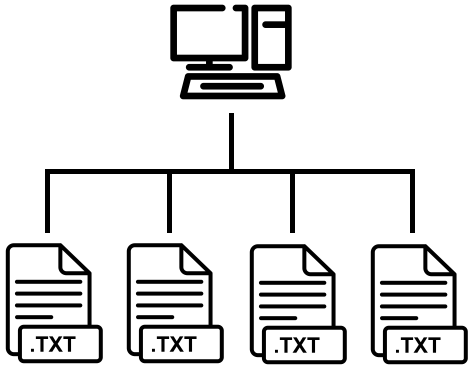
\includegraphics[scale = 0.7]{images/computer_to_txt_file_icon.png}
\caption{Database i form af tekst filer}
\end{figure}

I anden iteration er der gjort brug af en SQL relationel database, på baggrund af kravene til anden iteration. 